\chapter{Questionário}
\label{apendice:questionario}

As perguntas do questionário com suas respectivas respostas do questionário elaborado durante a etapa de elicitação de requisitos podem ser vistos nas Figuras ~\ref{q1} a ~\ref{q12}. O formulário pode ser acessado \href{https://forms.cloud.microsoft/r/uEDqVFwRvb}{neste link}.

\begin{figure}[H]
    \centering
    \caption{Número de Respostas e Tempo Médio.}
    
\includegraphics[width=0.7\textheight]{figuras/questionario/q1.png}
    \par
    Fonte: autoria própria.
    \par
    \label{q1}
\end{figure}

\begin{figure}[H]
    \centering
    \caption{Questão de Público Alvo.}
    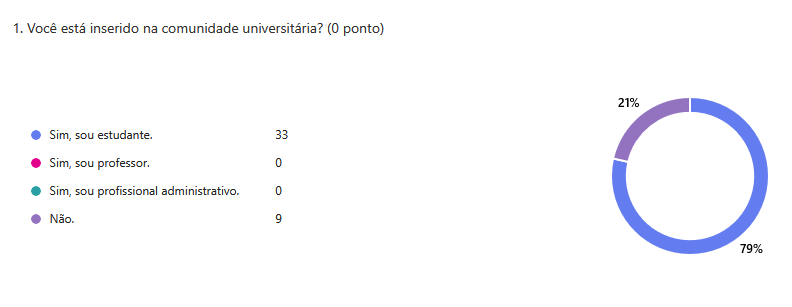
\includegraphics[width=0.7\textheight]{figuras/questionario/q2.png}
    \par
    Fonte: autoria própria.
    \par
    \label{q2}
\end{figure}

\begin{figure}[H]
    \centering
    \caption{Questão de permanência na comunidade universitária.}
    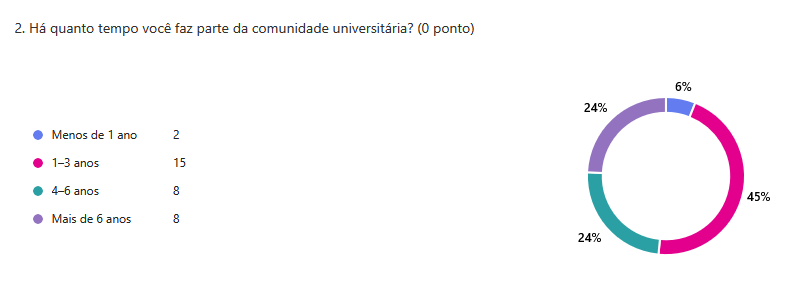
\includegraphics[width=0.7\textheight]{figuras/questionario/q3.png}
    \par
    Fonte: autoria própria.
    \par
    \label{q3}
\end{figure}

\begin{figure}[H]
    \centering
    \caption{Questão de Campus universitário.}
    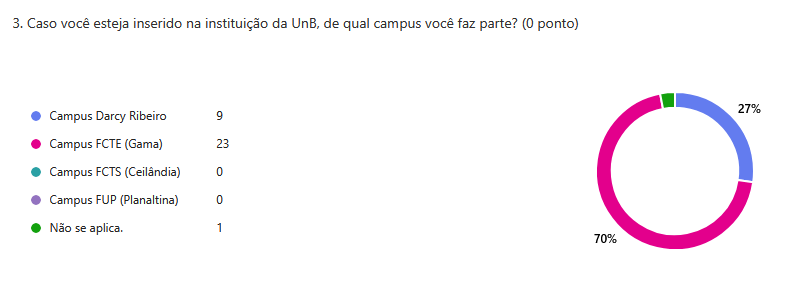
\includegraphics[width=0.7\textheight]{figuras/questionario/q4.png}
    \par
    Fonte: autoria própria.
    \par
    \label{q4}
\end{figure}

\begin{figure}[H]
    \centering
    \caption{Questões de Autoavaliação de hábitos.}
    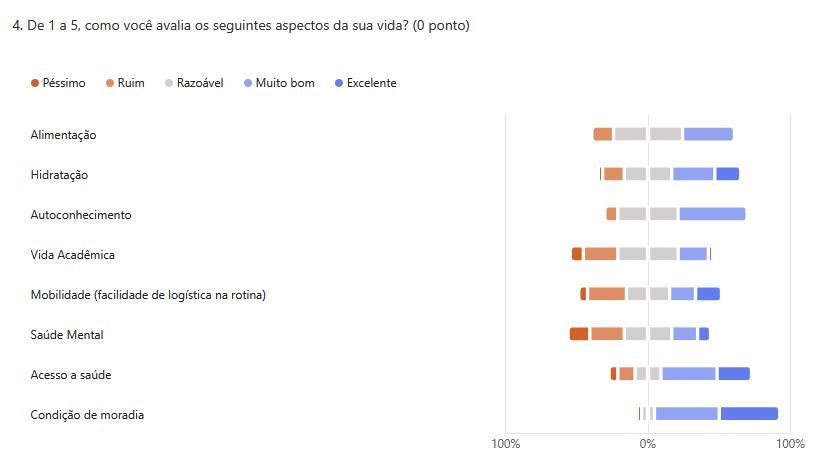
\includegraphics[width=0.7\textheight]{figuras/questionario/q5.png}
    \par
    Fonte: autoria própria.
    \par
    \label{q5}
\end{figure}

\begin{figure}[H]
    \centering
    \caption{Questões de Autoavaliação de frequência de hábitos.}
    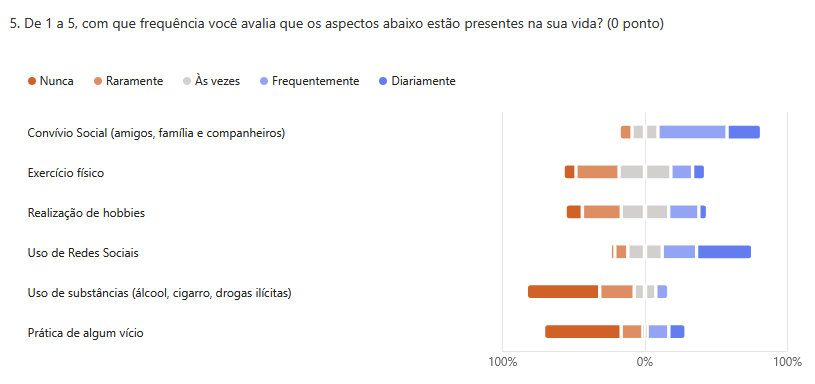
\includegraphics[width=0.7\textheight]{figuras/questionario/q6.png}
    \par
    Fonte: autoria própria.
    \par
    \label{q6}
\end{figure}

\begin{figure}[H]
    \centering
    \caption{Questões de Autoavaliação da saúde.}
    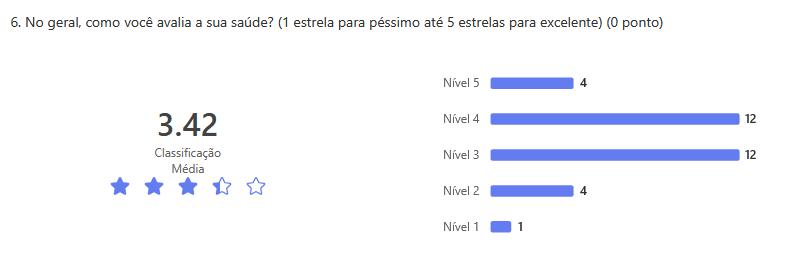
\includegraphics[width=0.6\textheight]{figuras/questionario/q7.png}
    \par
    Fonte: autoria própria.
    \par
    \label{q7}
\end{figure}

\begin{figure}[H]
    \centering
    \caption{Questões de demais tópicos do bem-estar.}
    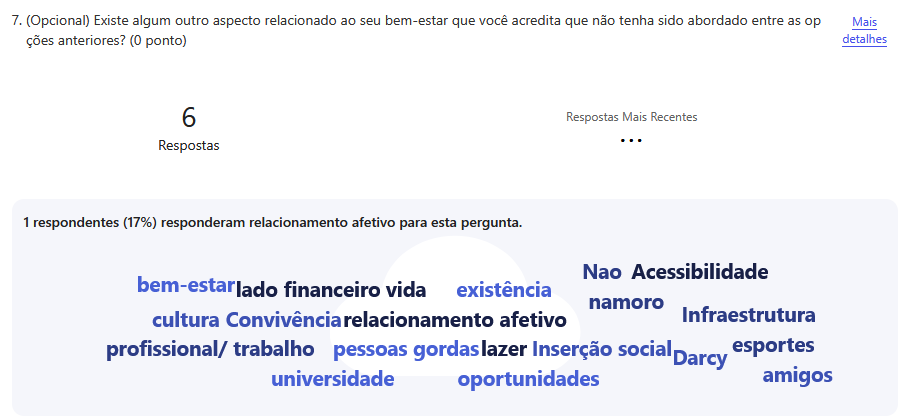
\includegraphics[width=0.6\textheight]{figuras/questionario/q8.png}
    \par
    Fonte: autoria própria.
    \par
    \label{q8}
\end{figure}

\begin{figure}[H]
    \centering
    \caption{Respostas de demais tópicos do bem-estar.}
    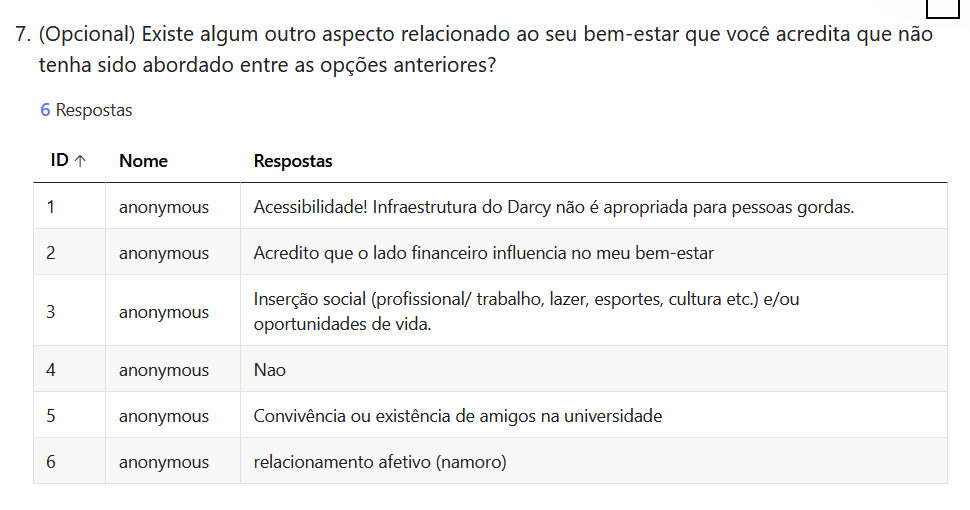
\includegraphics[width=0.7\linewidth]{figuras/questionario/qa.png}
    \par
    Fonte: autoria própria.
    \par
    \label{qa}
\end{figure}

\begin{figure}[H]
    \centering
    \caption{Questão de serviços de apoio a saúde nas instituições.}
    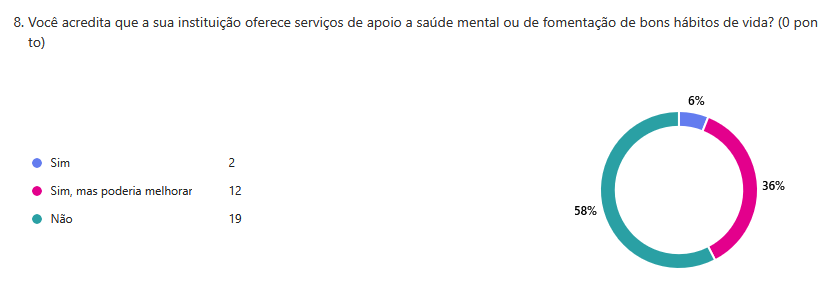
\includegraphics[width=0.6\textheight]{figuras/questionario/q9.png}
    \par
    Fonte: autoria própria.
    \par
    \label{q9}
\end{figure}

\begin{figure}[H]
    \centering
    \caption{Questão de aceitação de sistemas com foco em saúde.}
    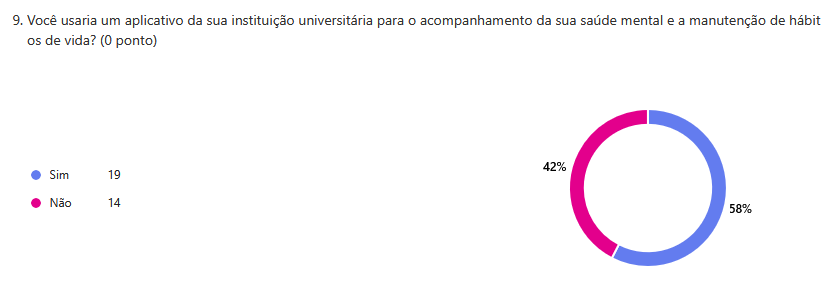
\includegraphics[width=0.6\textheight]{figuras/questionario/q10.png}
    \par
    Fonte: autoria própria.
    \par
    \label{q10}
\end{figure}

\begin{figure}[H]
    \centering
    \caption{Questão sobre funcionalidades do sistema.}
    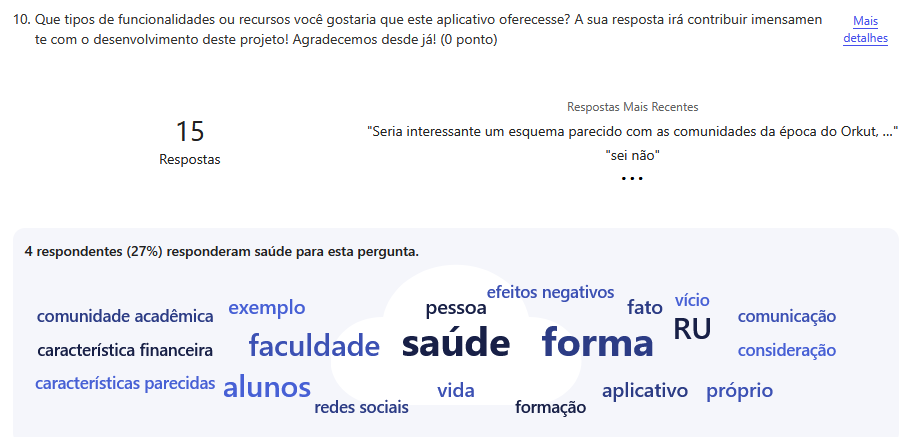
\includegraphics[width=0.6\textheight]{figuras/questionario/q11.png}
    \par
    Fonte: autoria própria.
    \par
    \label{q11}
\end{figure}

\begin{figure}[H]
    \centering
    \caption{Respostas sobre funcionalidades do sistema.}
    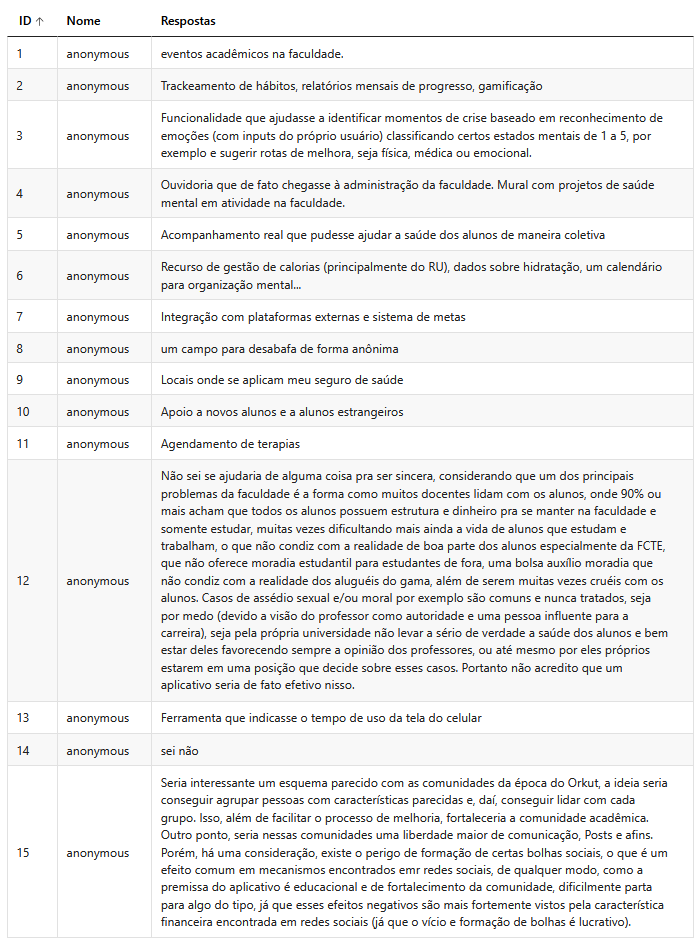
\includegraphics[width=0.7\textheight]{figuras/questionario/qb.png}
    \par
    Fonte: autoria própria.
    \par
    \label{qb}
\end{figure}

\begin{figure}[H]
    \centering
    \caption{Comentários adicionais.}
    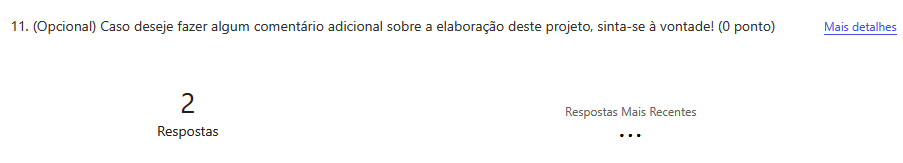
\includegraphics[width=0.6\textheight]{figuras/questionario/q12.png}
    \par
    Fonte: autoria própria.
    \par
    \label{q12}
\end{figure}

\begin{figure}[H]
    \centering
    \caption{Respostas nos comentários adicionais.}
    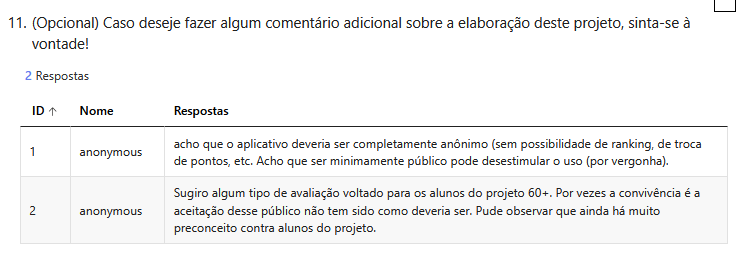
\includegraphics[width=0.6\textheight]{figuras/questionario/qc.png}
    \par
    Fonte: autoria própria.
    \par
    \label{qc}
\end{figure}